\chapter{Technology}


\section{Wombat}

\section{Python}

\section{C++}
\textbf{Author: Maximilian Dragosits}

C++ is a precompiled programming language that combines low-level memory management with support for object-oriented, generic, and functional programming paradigms. 
It was designed by Danish computer scientist Bjarne Stroustrup with a focus on efficiency, performance, and flexibility.\footcite{lecture_essence_cpp} C++ has 
become widely used in various domains, including desktop applications, servers, video games, and digital equipment for space exploration.\\

It was standardized by the International Organization for Standardization (ISO) in 1998 as ISO/IEC 14882:1998 and has since evolved into a powerful programming 
language. The popularity of C++ has led to the creation of numerous libraries and frameworks, such as Catch2\footcite{catch2_git} and Doxygen\footcite{doxygen_main_site}. 
These frameworks are essential to the project's development and functionality.\\

C++ was chosen as one of the two frontend languages for this project due to its impressive speed and efficiency, as well as the vast ecosystem of external 
frameworks and libraries already available. The resources are essential in developing the RECT library, improving the project's capabilities and accelerating 
the development process. The decision to use C++ was a strategic choice, aligning with the language's strengths and the abundance of tools and resources it 
offers to the development landscape.

\section{Rust}
\textbf{Author: Jeremy Sztavinovszki}

Rust is a general purpose multi paradigm programming language used in many fields ranging from embedded programming to web development. Although it is a relatively young language, having released its version 1.0 on May 15th 2015, it has seen great adoption from developers and has a big community. The language tries to be as fast as possibly, while still remaining memory-safe, which it achieves using its borrow checker. Even though it is possible to write unsafe code in Rust, that is not checked by the borrow checker, it is custom to keep the unsafe parts as small as possible.
Rust has a great ecosystem driven by the Rust Foundation and the Rust community. There are many tools, such as cargo, or rust-gdb, that provide great developer experience.
Right now there is now standardized async-runtime, so you normally use runtimes like tokio, async-std, or smol for programming asynchronously.

\section{gRPC}
\textbf{Author: Maximilian Dragosits}

gRPC\footcite{grpc_main_site} is an open-source framework that facilitates Remote Procedure Calls (RPC) across diverse environments. It is versatile 
and can be used in a broad spectrum of use cases, proving invaluable in establishing robust service-to-service connections. gRPC plays a pivotal role in the 
development of microservices and libraries. This framework is available in 11 different programming languages and provides developers with a flexible 
and accessible toolset for creating efficient and scalable communication channels.\\

gRPC's efficiency is central to its straightforward service definition and generation structure, which streamlines the integration process. 
This simplicity allows developers to focus on the core aspects of their projects, enhancing productivity and code maintainability. Furthermore, gRPC includes 
pluggable features such as authentication, load balancing, tracing, and health checking. These features provide developers with fine-grained control over 
service communication, ensuring robust and secure interactions within distributed systems.\\

In the context of the current project, gRPC plays a pivotal role. Its capability to seamlessly connect clients to backend services is particularly crucial. 
This feature enables efficient communication between Python and C++ frontends and the Rust backend, creating a cohesive and interoperable system. The project 
uses gRPC to achieve high communication efficiency, allowing for seamless data exchange between components and improving the overall performance and reliability 
of the system architecture.

\section{Protocol Buffers}
\textbf{Author: Maximilian Dragosits}

Protocol Buffers offer a platform-neutral solution for serializing structured data, similar to formats such as XML, JSON, or YAML. They provide a versatile 
solution that seamlessly interfaces with automatically generated source code across an array of programming languages, catering to developers' preferences. 
Noteworthy among the supported languages are Java, Kotlin, Python, and various C-based languages, underscoring the broad applicability of Protocol Buffers 
in diverse development ecosystems.\\

Protocol Buffers enable developers to efficiently manage and exchange structured data across different platforms and systems. They provide a unified approach 
to serialization, whether using the robustness of Java, the conciseness of Kotlin, the flexibility of Python, or the performance advantages of C-based languages. 
This approach promotes interoperability, enabling developers to easily incorporate serialized data into their projects, thereby enhancing the efficiency and 
maintainability of their codebases.\\

An example of a Protocol Buffer file illustrates the elegance and conciseness inherent in this technology, demonstrating its role in facilitating efficient 
data interchange.

\begin{verbatim}
    syntax = "proto3";
    package msg;
    
    
    message From {
      string conn_name = 1;
      string topic = 2;
    }
    
    
    message To {
      string conn_name = 1;
      string topic = 2;
    }
    
    
    message Msg {
      bytes data = 1;
      oneof fromto {
        From f = 2;
        To t = 3;
      }
    }
\end{verbatim}

As can be seen in this example the first part of any .proto file is the definition of the protobuf language version. Either \textit{proto2} or \textit{proto3}. Next the package within this will be 
stored in when it is converted into a programming languages code is defined. In this case it will be \textit{msg}. After that you can import any other .proto file.
Then it is possible to define any amount of the following types and many others not used by this project:
\begin{enumerate}
    \item \textbf{message:} Defines a special data structure that houses multiple variables of potentialy different data types, which can then be used in other enums or services.
    \item \textbf{enum:} Defines an enum which acts like the equivalent type of structure in other programming languages. This can then be used in other parts of then .proto file.
    \item \textbf{service:} Defines a Remot Procedure Call (RPC) system. The generated code for this will include service interfaces and stubs to be used by RPC frameworks.
\end{enumerate}

\subsection{Protofile message definition}

Message types in proto3 are relatively simple to define.

\begin{verbatim}
    message message_name {
        field_type field_name = number;
      }
\end{verbatim}

First the \textit{message} keyword is used to signify that the following is a declaration for a message type. Then a freely choose able \textit{message\_name} is 
used as the name for the later resulting message structure. After that any number of fields can be defined within the curly brackets. The \textit{field\_type} can be
one of multiple supported data types, which includes but is not limited to double, flout, integer, boolean, string as well as bytes. After defining an appropriate
\textit{field\_name} this format requires the assignment of a number between 1 and 536,870,911 to each field in a message. This is required in order to identify
the field after encoding.

There are also three other modifiers, that can be applied to fields:

\begin{enumerate}
    \item \textbf{optional:} If a field with this modifier does not have its value explicitly set later it will instead return a default value. It also possible to check if this it has been set.
    \item \textbf{repeated:} A field with this modifier can be repeated any number of times within the message and the order of the repetition will be saved.
    \item \textbf{map:} A field with this modifier acts like a key/value pair with the definition syntax being like that of a C++ map.
\end{enumerate}

Another way of defining fields, that can have a multitude or a currently unkown type, is to use either the \textit{any} or the \textit{oneof} types.
The \textit{any} type is then later resolved by Protobufs internal reflection code.
\textit{Oneof} is then automatically later defined as one of the given data types within curly brackets placed after the \textit{field\_name} is given.

\subsection{Protofile enum definition}

Enums are share a lot of the same traits as message types in terms of the defintion syntax.

\begin{verbatim}
    enum enum_name {
        constant_value = number;
    }
\end{verbatim}

Similarly to messages the enum is given an \textit{enum\_name} and then any number of \textit{constant\_value}s can be defined. All of these constants need an associated
value in order to function properly and the first of those needs to have 0 as its number, so that the enum has a default value in cases like fields with the \textit{optional}
modifier. 
In order to bind multiple \textit{constant\_value}s to the same \textit{number} the \textit{allow\_alias} option must be set to true. This is done by inserting this line
into the enum before any definition of \textit{constant\_value}s:

\begin{verbatim}
    option allow_alias = true;
\end{verbatim}

Once an enum is defined then it can be used in other parts of the Protocol Buffer, as seen in this example:

\begin{verbatim}
    enum Success {
        Ok = 0;
    }

    enum SendError {
        NoSuchConnection = 0;
        SendFailed = 1;
    }

    message SendResponse {
        oneof result {
            Success s = 1;
            SendError err = 2;
        }
    }
\end{verbatim}

\subsection{Protofile service definition}

Services allow the easy generation of service interfaces and stubs to then be used by RPC implementations.

\begin{verbatim}
    service service_name{
        rpc rpc_name(message_type) returns (message_type) {}
        rpc rpc_name(message_type) returns (stream message_type) {}
    }
\end{verbatim}

A service is defined with a \textit{service\_name} and after that any number of inidvidual methods. In order to define the methods first the keyword \textit{rpc} must be used.
Then a name for the method is given through \textit{rpc\_name} and a parameter for the \textit{message\_type} that this method accepts. And then a \textit{message\_type}
is defined as the return value of the RPC. A stream of a particluar \textit{message\_type} can be defined by putting the keyword \textit{stream} before the type.

An example of this would be the SubListen service from this project:

\begin{verbatim}
    service SubListen{
        rpc listen(ListenRequest) returns (ListenResult) {}
        rpc subscribe(ListenRequest) returns (stream ListenResult) {}
    }
\end{verbatim}

\section{Bluetooth Low Energy}
\textbf{Author: Jeremy Sztavinovszki}

Bluetooth Low Energy (BLE) is a low powered, low cost, low bandwidth radio communication technology, that was originally developed at Nokia in a project named Wibree. It was later noticed by the Bluetooth Special interest group and became part of the Bluetooth 4.0 Core Specification. Nowadays it is often used in all things ranging from wireless headphones to IOT devices and has seen great adoption in many different areas. The BLE protocol Stack, like others (e.g. TCP/IP) is separated into different layers. The layers are split into 3 overarching layers. which are the Application, Host and Controller layers.

\subsection{Application-Layer}
Much like the TCP/IP-Stack the BLE-Stack also comes with an Application-Layer. The Application-Layer is the highest layer in the stack and is responsible for containing logic, user interface and handling the data of the application using BLE. It often determines which usage model is used in the Host-Layers.
It is the layer that bundles all of the functionality of BLE together and abstracts it in such a way, that it is useable for ordinary users.

\subsection{Host-Layer}
The Host-Layer itself splits off into several layers. It is made up of all layers above the Host Side HCI, except the Application Layer, but not only that. It also contains profiles, which
determine how the protocols in the host layer should work with oneanother depending on the usage model, that has been chosen by the Application.

\subsubsection{Generic Access Profile GAP}
The Generic Access Profile, or GAP defines which role a BLE-Device has in communication. These roles determine how the device, as well as other devices act, when sending or receiving data.
A BLE device can take on 4 distinct roles, which are as follows.

\begin{itemize}
\item{Broadcaster}
\item{Observer}
\item{Peripheral}
\item{Central}
\end{itemize}


\subsubsection{Generic Attribute Profile GATT}
GATT

\subsubsection{Logical Link Protocol and Adaptation Protocol L2CAP}
L2CAP

\subsubsection{Attribute Protocol ATT}
ATT

\subsubsection{Security Manager Protocol SMP}
test

\subsubsection{Host Controller Interface HCI (Host side)}
test

\subsection{Controller}
The controller is the layer works closely with the hardware. It contains the following layers

\subsubsection{Host Controller Interface (Controller side)}
test

\subsubsection{Link Layer LL}
Hidden behind the HCI is the Link Layer. It is usually implemented as a conglomeration of custom hardware, as well as software it is the only part
of the protocol stack, that needs to have real-time capabilities, because it needs to work with the timing requirements defined by the specification.
In order to avoid overloading the CPU running the software layers of the stack, the easily automated, or computationally expensive parts are implemented in circuitry.


\subsubsection{Physical Layer PHY}
The physical layer is made up of the actual hardware, that is capable of modulating and demodulating the analog signals sent by radio and turning them into digital information. It uses the 2.4GHz ISM \footcite{ism} radio band, which it splits into 40 channels (37 for transmitting data and 3 for advertising connections and broadcasts) from 2.4GHz to 2.4835GHz. It uses FHSS to avoid radio interference, which is important, because classic bluetooth, as well as 2.4GHz use the same frequency band. The modulation rate chosen for BLE is 1.0Mbit/s, which means that is the physical throughput limit. However because of protocol overhead this physical throughput level is never reached.

\section{Libraries}

\subsection{Catch2}
\textbf{Author: Maximilian Dragosits}

Catch2\footcite{catch2_git} is a unit testing framework specifically designed for C++. It seamlessly integrates with C++ code and offers a testing environment 
that aligns closely with the overall structure of C++ code. Its ability to harmonize with the natural syntax of functions and boolean expressions is noteworthy. 
Catch2 not only facilitates unit testing but also incorporates micro-benchmarking capabilities, enabling developers to analyze performance in detail.\\

In the context of our project, Catch2 is an ideal choice for shaping the C++ frontend. Its integration into the development process ensures that unit tests 
become an integral part of the codebase, fostering a culture of code reliability and maintainability. In addition, the integration of micro-benchmarking in Catch2 
is consistent with our project's objectives, enabling thorough performance evaluations. This feature is essential in promoting optimizations, as benchmarks provide 
valuable metrics for measuring the speed and efficiency of implemented methods.\\

By using Catch2, our project benefits from a versatile testing framework that not only validates the functionality of the C++ frontend but also enables developers 
to make informed decisions about enhancements and optimizations. Catch2's seamless integration and benchmarking capabilities make it a valuable asset in ensuring 
the robustness, performance, and efficiency of the implemented methods within the project.

\subsubsection{Unit Tests}

Unit Tests in Catch2 are defined very similarly as normal functions in C++. This example, pulled from the Github repository of Catch2, shows the simplicity of
this framework and its integration into projects.

\begin{verbatim}
    #include <catch2/catch_test_macros.hpp>

    #include <cstdint>
    
    uint32_t factorial( uint32_t number ) {
        return number <= 1 ? number : factorial(number-1) * number;
    }
    
    TEST_CASE( "Factorials are computed", "[factorial]" ) {
        REQUIRE( factorial( 1) == 1 );
        REQUIRE( factorial( 2) == 2 );
        REQUIRE( factorial( 3) == 6 );
        REQUIRE( factorial(10) == 3'628'800 );
    }
\end{verbatim}

First the relevant Catch2 headers are included and then a function with a return value is defined. In this case it is the function factorial. 
This function will be executed by Catch2 during the testing process. Then a test case is a macro defined as:

\begin{verbatim}
TEST_CASE(string testname, string tags) {...test...}
\end{verbatim}

The argument \textit{testname} is a arbitrary name given to the unit test, which is then later during the running of the test printed alongside the results of the macro.
Tags can be given to the test by inputting one or multiple tags into the \textit{tags} field and change the behavior of the macro accordingly. In the case of the example above
the only given tag is the name of the function to be tested. After this the \textit{TEST\_CASE} macro has a curly brackets-enclosed body in which the logic of the test can 
be defined.\\
This requires the use of other specific macros included in the Catch2 framework. For example:

\begin{verbatim}
REQUIRE( function(value) == expected_value );
CHECK( function(value) == expected_value );
\end{verbatim}

The two macros described above, REQUIRE and CHECK, operate in a similar way. They both execute the given \textit{function} with the provided \textit{value} or \textit{values}
and then assert if the returned data equals true or false according to the provided boolean operator. If it does then it was successful and the rest of the \textit{TEST\_CASE} is executed. The difference 
between REQUIRE and CHECK is however that if a REQUIRE macro fails it throws an exception and the unit test is stopped from executing the remainder of code inside it.

\subsubsection{Micro-benchmarks}
The benchmarking macros in Catch2 are defined similarly to how unit tests are. Benchmarking in itself is a useful practice, that provides a way to measure the performance
and speed of a particular function.

\begin{verbatim}
#include <catch2/catch_test_macros.hpp>
#include <catch2/benchmark/catch_benchmark.hpp>

#include <cstdint>

uint64_t fibonacci(uint64_t number) {
    return number < 2 ? number : fibonacci(number - 1) + fibonacci(number - 2);
}

TEST_CASE("Benchmark Fibonacci", "[!benchmark]") {
    REQUIRE(fibonacci(5) == 5);

    REQUIRE(fibonacci(20) == 6'765);
    BENCHMARK("fibonacci 20") {
        return fibonacci(20);
    };

    REQUIRE(fibonacci(25) == 75'025);
    BENCHMARK("fibonacci 25") {
        return fibonacci(25);
    };
}
\end{verbatim}

In the example above the unit test macros and benchmark macros from Catch2 are first included in order to be used later. The function to be benchmarked is then defined
After that the TEST\_CASE macro is used combined with the [\!benchmark] tag in order to turn this unit test into a benchmark. In the actual body of the test the function
is first tested weather or not it actually works as intended before any benchmarks are done. This is done with the REQUIRE macro, since it throws an exception if the 
assertion fails, preventing the rest of the benchmark from executing unnecessarily. If all the tests before the benchmarks pass then the actual BENCHMARK macros are
executed.

\begin{verbatim}
BENCHMARK(string name) {
    ... benchmark ...
};
\end{verbatim}

As part of the BENCHMARK macro a arbitrary name is given to it, which is then later during the output of the test used as a identifier for the specific benchmark.
Then the actual logic of the benchmark is then defined within curly brackets giving a lot of freedom in how a certain benchmark is executed. Adding a return statement
within the benchmark will ensure that the compiler doesn't mess with the test.\\
\vspace{\baselineskip}
After this is run a summary is automatically output within the command line window. This includes multiple data points that pertain to the execution speed of the tested
function:
\begin{enumerate}
    \item \textbf{Samples:} The amount of times the code within the curly brackets of the BENCHMARK macro is repeated in order to build a dataset to calculate the mean execution time.
    \item \textbf{Iterations:} %Need to find out what this is
    \item \textbf{Estimated run time:} The estimated amount of time the code within the benchmark will take to run. Mesured in milliseconds.
    \item \textbf{Mean/low mean/high mean run time:} The mean time it will take for the code to run as well as the low mean and high mean for this in nanoseconds.
    \item \textbf{Standard deviation:} The standard deviation from the mean time in nanoseconds,
\end{enumerate}

\subsection{Doxygen}
\textbf{Author: Maximilian Dragosits}

Doxygen\footcite{doxygen_main_site} is a versatile C++ framework that automates the generation of documentation for C++ code. It can also be used for other programming languages such as 
PHP, Java, Python, IDL, and Fortran. Doxygen extracts information directly from annotated source code, making the documentation process more efficient and 
accessible for developers.\\

Doxygen is notable for its flexibility in delivering documentation. The generated documentation can be accessed online through an HTML website or offline 
through a LaTeX document, providing options tailored to developers' preferences. Additionally, Doxygen can derive structure overviews even from non-annotated 
sources, facilitating a holistic understanding of the codebase. The project's architecture can be visualized more effectively by displaying entity relations 
through insightful graphs.\\

A quick overview of a Doxygen implementation shows a well-organized framework that streamlines the documentation process. This implementation improves code 
comprehension and promotes a collaborative development environment by providing a centralized repository of project documentation. The image shows how Doxygen's 
integration simplifies and enhances the documentation workflow, contributing to the clarity and accessibility of the project.\\

\begin{figure}[h]
	\centering
	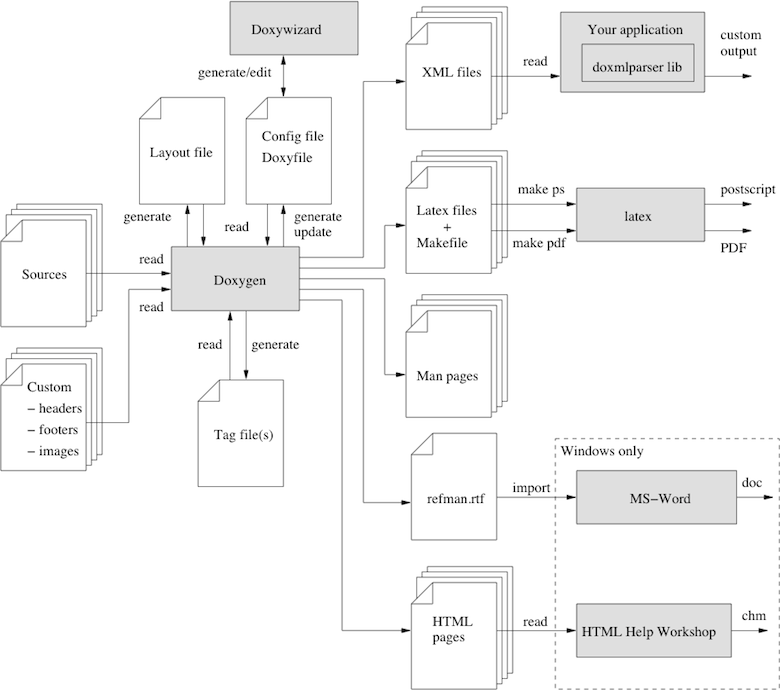
\includegraphics[width=\textwidth]{doxygenInfoflow.png} 
	\caption{Doxygen Infoflow diagramm\footcite{doxygen_main_site}}
	\label{pic:doxygenInfoflow}
\end{figure}

First a Doxygen config file, also called a \textit{Doxyfile} is generated in a project using the \textit{Doxywizard} and can be edited using this tool afterwards. 
This file is later read and updated during the generation process from \textit{Doxygen}. The layout files and tag files are also generated and used by \textit{Doxygen}
to facilitate the creation of the documentation.\\
\vspace{\baselineskip}
\textit{Sources} are the files with the actual source code, that will be part of the documentation, in them. These files are read alongside any other additional \textit{Custom}
files. For example the headers for source code, footers for the following document or images to be used in it. There are of course many other files that can be included
in order to refine the result further.\\
\vspace{\baselineskip}
Finally \textit{Doxygen} uses all this to generate documentation in the specified formats: XML, LaTex, Man, refman or HTML. \\

\subsubsection{Doxygen Configuration}
The first step in creating documentation with Doxygen is a configuration file. This can be automatically generated by the \textit{Doxywizard} with this command:

\begin{verbatim}
    doxygen -g <config-file>
\end{verbatim}

In this example \textit{<config-file>} is a stand-in for the name of the generated configuration file. There are many tags within this config file that change how 
the end result will look and what sources should be used or ignored. For example the INPUT tag specifies the location that \textit{Doxygen} will search for code and
EXCLUDE forbids it to use files contained within the given directories. After editing the file using a text editor or Doxywizard this command can be used to generate 
the documentation.

\begin{verbatim}
    doxygen <config-file>
\end{verbatim}

Doxygen normally requires the source code to be annotated in order to generate documentation, but a rough version can be made by setting the tag EXTRACT\_ALL to YES.
This will extract even the non-annotated classes and functions from the source code.

\subsubsection{Doxygen Annotation}

If the EXTRACT\_ALL tag is not enabled then the classes, functions and members within the source files need to be annotated in order to be picked up by \textit{Doxygen}
and turned into a documented section. There are many ways of signaling to \textit{Doxygen}, that you want it to produce documentation from a source. In general there
are two ways to do this:
\begin{enumerate}
    \item \textbf{Documentation within source:} In this way of annotation special comment blocks are inserted before and after parts of the source code. 
                This will cause the text within this special block to be displayed alongside the class, function, or member within the documentation.
    \item \textbf{Documentation outside source:} In this way of annotation the special comment blocks are written within a separate file and then connected 
                to the sources by way of a reference. With this method references to the source file need to be written within this distinct file.
\end{enumerate}

In \textit{Doxygen} special comment blocks are similar to C++ comments, but with extra characters in order to be picked up during generation. There are many different 
ways to define special comment blocks:\\
\vspace{\baselineskip}
\textbf{Javadoc and Qt style:} This way a special block can be definied just like a multi line comment in C++ with a special character after the first *.
\begin{quote}
\begin{verbatim}
    /**
     *   ... text ...
     */
\end{verbatim}
Or:
\begin{verbatim}
    /*!
     *   ... text ...
     */
\end{verbatim}
\end{quote}      
\vspace{\baselineskip}
\textbf{C++ comment style:} This style is similar to a C++ single line comment with an added / or ! at the begining.
\begin{quote}
\begin{verbatim}  
    ///
    ///  ... text ...
    ///
\end{verbatim}
Or:
\begin{verbatim}
    //!
    //!  ... text ...
    //!
\end{verbatim}
\end{quote}
\vspace{\baselineskip}
\textbf{Visible style:} This is a more clearly visible version of the previous two styles.
\begin{quote}
\begin{verbatim}
    /************************************
     *   ... text ...
    ************************************/
\end{verbatim}
Or:
\begin{verbatim}
    //////////////////////////////////////
    ///  ... text ...
    //////////////////////////////////////
\end{verbatim}
\end{quote}
\vspace{\baselineskip}

In documentation outside of the source additional commands are required. At the start of the document file a special comment block needs to have the name of the
file to be documented referenced by putting a backslash or an @ symbol before the filename in the first line of the block. After that any number of other 
special comment blocks can be defined with the first line in each of them being used to reference the desired class, function, member, struct, etc. This is done by
first using the equivalent structural commands and then inserting the definition statement of the chosen object. This can be seen in this example:\\

\begin{verbatim}
    /*! \fn int open(const char *pathname,int flags)
        \brief Opens a file descriptor.

        \param pathname The name of the descriptor.
        \param flags Opening flags.
    */
\end{verbatim}

In this case \textit{fn} is the structural command, which tells \textit{Doxygen} what type the object is.\\
\vspace{\baselineskip}

The other structural commands that can be seen in this example can be used in both documentation inside sources and outside sources. Using the \textit{brief} command 
is used to give a short description to the object and \textit{param} in order to signify and describe the parameters of this function.\\

\subsubsection{Doxygen Parsing}

During the documentation generation process, Doxygen parses special comment blocks and translates them into various output formats to create comprehensive 
documentation. The parser performs several key processes, culminating in the creation of documentation with Doxygen.

\begin{itemize}
    \item[] One of these processes is the conversion of Markdown writing within comment blocks into HTML, ensuring compatibility with web-based documentation platforms. This conversion improves the presentation of textual content, making it more accessible and visually appealing.
    \item[] Special commands embedded within the comment blocks are executed, allowing developers to include custom instructions or annotations. This feature empowers developers to tailor the documentation to specific project requirements, fostering flexibility and customization.
    \item[] Blank lines are handled appropriately. Paragraph separators are strategically used instead of blank lines to enhance the readability and organization of the generated documentation. This helps developers to better understand the information presented.
    \item[] Doxygen generates links to other sections of the documentation based on special comment blocks. The interlinking mechanism enables smooth navigation within the documentation, improving the user experience and promoting a cohesive understanding of the codebase.
    \item[] In situations where the output format is LaTeX, Doxygen converts HTML elements within the comment blocks into LaTeX commands. This transition ensures consistency and compatibility when generating LaTeX documents. It allows developers to choose the format that best suits their documentation needs.
\end{itemize}


\subsection{Rusqlite}
\textbf{Author: Christoph Fellner}

Rusqlite is an ergonomic wrapper for using SQLite from Rust similar to rust-postgres. It provides an easy-to-use interface to work with SQLite databases. Using the functions provided by rusqlite you can perform all the common database operations, such as creating tables, inserting Data, querying data, and more simply within your code. 
We choose this library for SQLite mainly because of three reasons:
\begin{enumerate}
    \item \textbf{Portability:} SQLite databases can be used across different platforms and operating systems. Given the fact that RECT operates on different small Controllers, portability is very important.
    \item \textbf{Configuration:} There is no need for any complex setup or configuration when working with SQLite. We only need a few tables to work with, so having to configure a database on each controller wouldn't be worth the effort.
    \item \textbf{Local:} SQLite doesn't need any separate server or installation. It contains all the features we need in a small an independent package.
\end{enumerate}

In our case we use rusqlite in order to save the config.json file, containing date for the available connections. Accessing the Data from the database is simply much quicker and saver than reading from the file when we need it. 

\subsection{Serde}
\textbf{Author: Christoph Fellner}

Serde is a framework for rust, used for \textbf{ser}ializing and \textbf{de}serializing data structures efficiently and generically. You can find a detailed serde overview \href{https://serde.rs/}{here}.

Serde provides functions to deserialize JSON-files in a simple and quick way, this allows us to use the data from the config.json file in our program with just a few lines of code.

With serde we deserialize the data from the JSON-file into a self-made rust structure, which allows us to use the data properly.  

\subsection{Tokio}
\textbf{Author: Christoph Fellner}

Tokio is asynchronous runtime for rust. In rust asynchronous code doesn't run on it's own in order to make it work the programmer has to use a runtime like Tokio. You can find more in depth descripton of Tokio \href{https://tokio.rs/tokio/tutorial}{here}. 

We picked Tokio because it is the most widely used runtime for async rust code. There are also a lot of Tutorials for Tokio and it is fairly simple to use.

Tokio as our asynchronous runtime allows us to execute multi-threaded async code safely.  

\subsection{Tonic}
\textbf{Author: Christoph Fellner}

Tonic is a rust framework that implements gRPC.

\filbreak
